% !TEX root =  main.tex
\section{Results}
  We implemented our algorithm, which we will refer to as \textbf{asx}, for sparse matrices in CSR format. Because the competing algorithm, which we will refer to as \textbf{oski} described in \cite{VuducDeYe05} was implemented in C, we implmented our algorithm in C as well. To remove differences in speed from using different library functions, we modified the algorithm from \cite{VuducDeYe05} to use the default GSL random number generator, which is an implmentation of the \texttt{mt19937} mersenne twister \cite{mt19937}, a pseudorandom number generator which is considered suitable for use in monte carlo simulations.

  To avoid differences in speed due to different integer types, we stored all indices in the sparse matrix using the unsigned type $size_t$, a macro which expands to a 64-bit unsigned quantity on our system.

  The implementation of the \textproc{Sample} subroutine followed the pseudocode, but we had to get creative when implmenting \textproc{NonzerosInRange}... More on this later...

  In practice, we found that the runtime and accuracy of the oski implementation varied substantially across matrices, even for the same parameter settings. Ideally, sampling algorithms should be able to provide users with a consistent level of accuracy so that they can use the estimates provided with some confidence. The variance in oski's runtime made it difficult to create useful plots. Despite this difficulty, almost all sampling algorithms, including oski, provide some tradeoff between accuracy and runtime. Even though the relationship between oski's parameters and its runtime and accuracy is unpredictable, the relationship between oski's runtime and its accuracy is familiar. Therefore, we show, for both asx and oski, the error in the estimates after running these methods for differing lengths of time. The error shown is the median of 100 runs, and the time shown is mean of the same 100 runs. The error bars reflect one standard deviation of the measured errors above and below the estimates.

  I don't have time to make a nice results section right now, but our method works. Check out these plots:


  \begin{figure}
  \centering
  \begin{subfigure}{.5\textwidth}
    \centering
    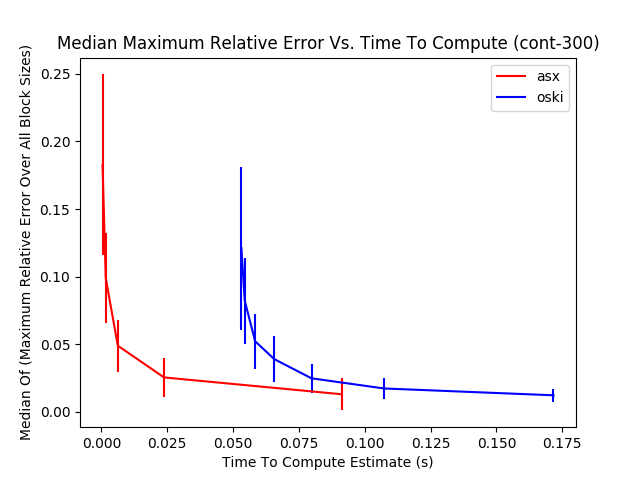
\includegraphics[width=1.0\linewidth]{../code/roi_cont-300.png}
    \caption{Results on a matrix}
    \label{fig:sub1}
  \end{subfigure}%
  \begin{subfigure}{.5\textwidth}
    \centering
    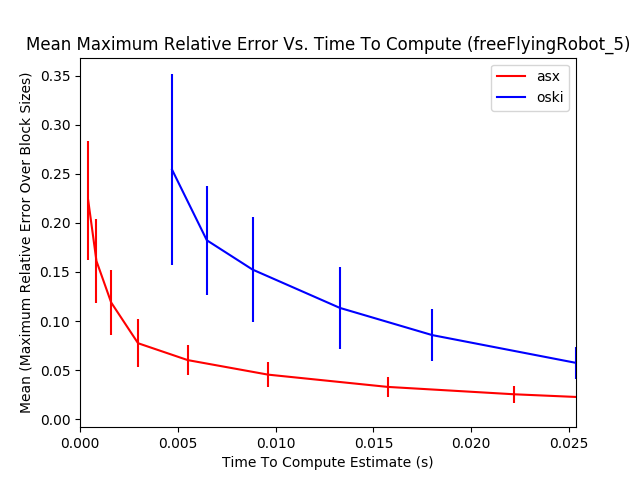
\includegraphics[width=1.0\linewidth]{../code/roi_freeFlyingRobot_5.png}
    \caption{Results on a different matrix}
    \label{fig:sub2}
  \end{subfigure}
  \caption{Our results}
  \label{fig:test}
  \end{figure}

  Because oski samples entire rows, its accuracy and runtime depend on the shape of the matrix. Therefore, we compare the performance of asx and oski on a short fat matrix ($512 \times 8192$), a square matrix ($2048 \times 2048$), and a tall, skinny matrix ($8192 \times 512$) where nonzeros are randomly included with probability $1/12$. 


  \verb|http://www.math.sci.hiroshima-u.ac.jp/~m-mat/MT/MT2002/emt19937ar.html|

